\documentclass[sigconf]{acmart}
\settopmatter{printacmref=false, printccs=false, printfolios=true}
\renewcommand\footnotetextcopyrightpermission[1]{}
\setcopyright{none}
\setlength{\emergencystretch}{1.5em} % avoids overfull lines with long \texttt names

\usepackage{booktabs} % For formal tables
\usepackage{pgfplots}
\pgfplotsset{compat=1.18}
\usepackage{xurl} % lets the long Spark configuration names break across lines


\begin{document}
\title{Large-Scale Analytics with Spark}
\subtitle{Profiling and Optimising a PySpark Pipeline over the NYC Yellow Taxi Records}

% TODO: confirm names, emails and affiliation
\author{Miguel Lan\c{c}a}
\email{TODO@domain.com}

\author{Pedro Marteleira}
\email{TODO@domain.com}


\begin{abstract}
This report describes the implementation, profiling and optimisation of a PySpark pipeline over
the NYC TLC Yellow Taxi trip records, this pipeline ingests and cleans the raw records, calculates
the temporal demand per borough and monthly statistics per zone with window functions, and
implements three of the optional modules: fare anomalies, demand forecasting features and
trip type classification, all experiments performed were conducted on a Spark~4.2 standalone cluster
running with Docker on a single laptop, over the complete year of 2019 (with 84.6\,M records).
Starting from a very simple baseline, we identified three bottlenecks in the query plans and event
logs, namely the recomputation of the input, the shuffle of the whole trip table and a join placed
before an aggregation, and then we addressed each one with a measured change, the final version of the pipeline is 42\%
faster than the baseline and shuffles 97\% less data. The strong scaling, on the other hand, is
limited by the environment itself, since every worker shares the same four physical cores of the machine.
\end{abstract}

\keywords{Apache Spark, PySpark, performance profiling, query optimisation, scalability}


\maketitle
\pagestyle{plain} % no "Conference'17" running headers

\section{Introduction}

Apache Spark~\cite{zaharia2016spark} is nowadays the reference engine for the processing with
large datasets, in great part due to the powerful DataFrame API of Spark SQL~\cite{armbrust2015sparksql},
whose optimiser decides the most of the physical execution, however a correct Spark program is not
necessarily an efficient one, since the same analysis may read the input several times, move gigabytes
across the network or run hundreds of tiny tasks, depending on decisions that are not visible in
the source code.
In this work assingment we implemented a pipeline over the NYC TLC Yellow Taxi trip records~\cite{tlc},
composed of the mandatory operations (M1 to M3) and three of the optional operations (O1, O3 and O4). We
followed a strict methodology: first, a simple baseline thought AI agents, without caching, broadcast hints or
configuration tuning, then the profiling of the baseline with the Spark UI, the physical plans
and the event logs, and only after that the optimisations, one at a time, and each one measured against
the previous version. 

Section~\ref{sec:design} describes the implementation,
Sections~\ref{sec:baseline} and~\ref{sec:optimisations} the profiling and the optimisations,
Section~\ref{sec:analysis} the scalability analysis, and Section~\ref{sec:conclusion} concludes.


\section{Pipeline Design}
\label{sec:design}

This pipeline is organised as one Python package per operation, and a single entry point only
creates the session, calls each operation and writes its result, there are two rules that were followed
throughout the code: firstly, the modules contain no actions (\texttt{count}, \texttt{collect},
\texttt{show}): each operation ends in exactly one Parquet write and, since everything before it
is lazy, the duration of that write is the duration of the operation, secondly, no Python User-defined-functions (UDFs)
are used, so every expression can be optimised by Catalyst and no data has to be serialised
between the JVM and the Python workers. The session time zone is set to UTC, to match the
timestamps stored in local New York time, and are never shifted by the time zone of the executors.


\paragraph{Ingestion and cleaning (M1)}
The schema of the files is not stable across the years, since some columns change the case of their
name (i.e.\ \texttt{airport\_fee}) or a change from an integer to double, and a single
\texttt{spark.read.parquet} over all the files fails, for this reason the files are grouped by
the physical schema (only the Parquet footers are read), each group is mapped onto a canonical schema
of 20 columns by a case-insensitive name match followed by an explicit cast and the groups are
combined with \texttt{unionByName}, the surcharges that did not exist in the earlier years are
set to zero, since their absence means that they are not charged, and the files of 2009 to 2010,
which have coordinates instead of location IDs, are discarded.
A record is invalid when it violates at least one of five rules, null values counting as violations: non-positive fare or distance, 
\texttt{passenger\_count} outside 1--6, drop-off not after the pickup,
and pickup or drop-off location outside 1--263 (264 and 265 are the \emph{unknown} and
\emph{outside of NYC} zones). The rules of the validations are kept as SQL conditions in a dictionary, so the
filter and the per-rule statistics (one pass, behind a \texttt{--stats} flag) share the same definition. 
In the year of 2019, about 80.8\,M of the 84.6\,M records (95.5\%) are valid.

\paragraph{Temporal demand and zone statistics (M2 and M3)}
The M2 joins the trips with the zone lookup on the pickup side and computes, per
(\texttt{pickup\_borough}, \texttt{day\_of\_week}, \texttt{hour\_of\_day}), the number of trips
and the mean fare, duration and distance and the output is partitioned by borough. 
In the M3, a\emph{month} is a calendar month of a given year, so for example January 2019 and January 2020 are
different.
For the per (zone, month) we compute the mean and sample standard deviation of the fare and
distance and the rank of the zone by volume inside its borough using window functions, the
rolling 3-month trip share, i.e.\ the trips of the zone in the current and two previous months
over those of its borough in the same period, and an anomaly flag raised when the volume deviates
from the mean of the three \emph{previous} months by more than 1.5 standard deviations. The
windows use \texttt{rangeBetween} over a month index instead of \texttt{rowsBetween}, so a \emph{month} without trips is not silently skipped.

\paragraph{Optional operations (O1, O3 and O4)}
The O1 calculates the fare per mile of every trip and its mean and the standard deviation per (pickup zone,
hour), a trip is anomalous when it exceeds the mean by more than $3\sigma$, these statistics are
joined back to every trip, and the anomaly rate is aggregated by the day type (weekday or weekend),
payment type and borough. 
The O4 computes per (pickup zone, hour), the fraction of airport trips
(\texttt{RatecodeID} 2 or 3), of the negotiated fares (\texttt{RatecodeID} 5) and of group trips
(4 or more passengers), and labels the bucket as \emph{transit}, \emph{commercial} or
\emph{residential} when the respective fraction reaches a configurable threshold, or as \emph{mixed} otherwise.
The thresholds (0.10, 0.35 and 0.12) are close to the 90th
percentile of each fraction in January 2019, so the top 10\% of the buckets receive
each label, the label is joined back to every trip, and the trips are aggregated per zone type
and month. 
Finally, the O3 counts the trips per (zone, date, hour) and calculates the mean and variance
of these counts per (zone, day of week, hour) over the loaded period, the count of four weeks
before is obtained through a self-join with the date shifted by 28 days (a left join, since the
first four weeks have no lag), the slots whose count is more than twice the bucket mean are
flagged as demand spikes, and each slot is annotated with the \texttt{service\_zone} of its zone,
the hours without any trips haven't any row, which is a simplification since the bucket means of the quiet zones are
slightly overestimated.

% results.tex -- Profiling and Baseline, Optimisation Study, Analysis
% Every number comes from report/results/benchmark.csv and stages.csv (bench/benchmark.sh).
% Times are medians of 3 interleaved runs unless stated otherwise.
% Needs \usepackage{booktabs} and \usepackage{pgfplots} (\pgfplotsset{compat=1.18}) in the preamble.

\section{Profiling and Baseline}
\label{sec:baseline}

\paragraph{Setup.}
No DI cluster was available, so every experiment ran on one laptop (Intel i5-8365U,
4 cores / 8 threads, 16\,GB RAM, Windows~11) with a Spark~4.2.0 standalone cluster in Docker
(WSL2, Java~21): one master and two workers with 2 cores each, i.e.\ 4 task slots.
The input is the full year 2019 (12 files, 1.2\,GB of Parquet, 84.6\,M records), as allowed by
the assignment when no cluster is available. Each executor gets 2\,GB
(\texttt{--executor-memory 2g}, see Section~\ref{sec:opt-memory}); the only other non-default
setting is \texttt{spark.sql.optimizer.canChangeCachedPlanOutputPartitioning=true}
(Section~\ref{sec:opt-cachedaqe}). Every operation ends in one Parquet write, so the time of that
write is the time of the operation. Stage metrics (tasks, shuffle bytes, spill, task-time
skew) are extracted from the Spark event log of every run. Versions are measured in
interleaved rounds (A, B, C, A, B, C, \dots) on mains power with the \emph{best performance}
power mode; the run-to-run spread of the wall time is up to $\pm$10\% (laptop thermals), so
smaller differences are not claimed as gains.

\paragraph{Baseline.}
The baseline completes in \textbf{341.7\,s} (median, runs from 314.2 to 370.7\,s);
Table~\ref{tab:baseline} breaks it down per operation.

\begin{table}[h]
  \caption{Baseline per operation (2019, 2 workers, median of 3 runs).}
  \label{tab:baseline}
  \small
  \begin{tabular}{lrrrr}
    \toprule
    Op & Time (s) & Tasks & Records read (M) & Shuffle write (MB) \\
    \midrule
    M2 & 45.1 & 14 & 84.6 & 0.7 \\
    M3 & 40.3 & 18 & 84.6 & 1.4 \\
    O1 & 85.1 & 53 & 169.2 & 1{,}320.9 \\
    O4 & 83.1 & 38 & 169.2 & 1{,}284.8 \\
    O3 & 76.4 & 48 & 169.2 & 98.9 \\
    \midrule
    Total & 341.7 & 184 & 676.8 & 2{,}707 \\
    \bottomrule
  \end{tabular}
\end{table}

The event logs and plans point to three bottlenecks:
\begin{enumerate}
  \item \textbf{Recomputation.} Nothing is cached, so the Parquet scan and the cleaning
    filter run 8 times (once in M2 and M3, twice in O1, O4 and O3): 676.8\,M records are read
    for an 84.6\,M-record input.
  \item \textbf{Shuffling the whole trip table.} O1 and O4 join every trip back to a
    $\sim$6\,k-row table of (zone, hour) statistics with a \texttt{SortMergeJoin}, which
    shuffles 1.3\,GB each; together they account for 96\% of all shuffle bytes.
  \item \textbf{M3 joins before aggregating.} The zone lookup is joined to all 84.6\,M
    trips before the \texttt{groupBy}, although the borough and zone only depend on
    \texttt{PULocationID}.
\end{enumerate}
We also looked for the other symptoms listed in the assignment and did not find them: the
\texttt{FileScan} reads only the 9 columns used (of 20), with \texttt{IsNotNull} filters pushed
down; no stage spills to disk; and no stage has skewed tasks (the slowest task is at most
2.0$\times$ the median in every stage longer than 0.5\,s, far from the 10$\times$ threshold).
Finally, every 2019 file is a single Parquet row group of 7--8\,M rows, so the scan is fixed at
12 tasks for 4 slots (3 waves) whatever \texttt{maxPartitionBytes} is.

\section{Optimisation Study}
\label{sec:optimisations}

\subsection{Executor memory}
\label{sec:opt-memory}
\textit{Observation.} With the default 1\,GB executors the baseline runs, but every version that caches the cleaned trips fails with \texttt{OutOfMemoryError} while the
cache is being built (\texttt{InMemoryRelation} / \texttt{MemoryStore.putIterator}), after 4
retries of the same task. \textit{Hypothesis.} Each task caches a whole month (one row
group, $\sim$7\,M rows) and two tasks share a 1\,GB heap. \textit{Change.}
\texttt{--executor-memory 2g} for all versions, including the baseline (2 executors of
2\,GB fit the 7.7\,GB Docker VM). \textit{Result.} The cached versions complete; this setting is
used for every number in this report.

\subsection{Caching the cleaned trips}
\label{sec:opt-cache}
\textit{Bottleneck.} Recomputation: 8 scans, 676.8\,M records read (Table~\ref{tab:baseline}).
\textit{Hypothesis.} Persisting the cleaned trips once (\texttt{MEMORY\_AND\_DISK}) replaces 7
of the 8 scans by reads of the cache. \textit{Change 1.} Persist the cleaned DataFrame as is.
This \emph{fails}: the cached rows still hold all 20 columns and the executors run out of heap
even with 2\,GB. \textit{Change 2.} Select the 8 columns the analyses use before persisting.
\textit{Result.} The cache takes 1{,}463\,MB, all 12 blocks in memory, and the input is read
once (84.6\,M records). The wall time drops from 341.7 to \textbf{207.9\,s (-39\%)}. M2 becomes
slower (45.1$\rightarrow$92.4\,s) because it now pays for building the cache, while the
following operations become 2--4$\times$ faster (M3 40.3$\rightarrow$22.6, O1
85.1$\rightarrow$33.1, O4 83.1$\rightarrow$26.7, O3 76.4$\rightarrow$21.8\,s). Because
Change~1 never completes, this measurement also includes the broadcast joins of
Section~\ref{sec:opt-broadcast}, which were committed together with it.

\subsection{Broadcast joins in O1, O4 and O3}
\label{sec:opt-broadcast}
\textit{Bottleneck.} \texttt{SortMergeJoin} of all trips with the (zone, hour) statistics:
1{,}321\,MB (O1) and 1{,}285\,MB (O4) of shuffle. \textit{Hypothesis.} The statistics table has
at most 265 zones $\times$ 24 hours rows, so sending it to every executor is cheaper than
shuffling 84.6\,M trips. \textit{Change.} \texttt{sf.broadcast()} on the statistics side of the
O1 and O4 joins, and on the bucket statistics of O3. \textit{Result.} Shuffle write drops to
3.1\,MB in O1 and 1.5\,MB in O4; over the whole pipeline from 2{,}707 to 72\,MB (-97\%). The
time gain is part of the -39\% above.

\subsection{Aggregating before the join in M3}
\label{sec:opt-m3}
\textit{Bottleneck.} M3 joins the zone lookup to every trip before grouping by zone and month.
\textit{Hypothesis.} Grouping by \texttt{(PULocationID, month)} first and joining the 265-row
lookup to the $\sim$3\,k aggregated rows gives the same result with a much smaller join.
\textit{Change.} Swap the order. (The window functions were also reordered so that the two
windows partitioned by borough can share one exchange; on $\sim$3\,k rows any effect is
negligible.)
\textit{Result.} M3 goes from 22.6 to \textbf{13.6\,s (-40\%)}. The wall time goes from
207.9 to 196.7\,s, which is within the run-to-run spread, so we only claim the per-operation
gain.

\subsection{Re-planning cached plans with AQE}
\label{sec:opt-cachedaqe}
O3 also caches its hourly counts, which are the output of a shuffle, and reads them three times
(bucket statistics, current slots, 4-week lag). The pipeline enables
\texttt{canChangeCachedPlanOutputPartitioning} (default \texttt{false}). \textit{Hypothesis.}
We expected no effect, since the main cache comes straight from the Parquet scan, and measured a
version without the setting. \textit{Result.} The hypothesis was wrong: without it the cached
counts keep the default 200 shuffle partitions, because AQE may not coalesce a cached plan, and
O3 runs 6 stages of 200 tasks of 30--100\,ms each (1{,}217 tasks instead of 44). O3 takes
67.1\,s instead of 22.5\,s and the pipeline 236.8\,s instead of 199.4\,s. The setting is kept.

\subsection{AQE settings that were already defaults}
\label{sec:opt-aqe}
The pipeline also set \texttt{adaptive.enabled}, \texttt{coalescePartitions},
\texttt{skewJoin} and \texttt{localShuffleReader} to \texttt{true}, to handle skew. Spark~4.2
already uses these values by default (checked with \texttt{spark.conf.get}), and the profile
shows no skew, so they were removed. As expected the wall time does not change (196.7\,s before,
199.4\,s after).

\subsection{Summary}
Table~\ref{tab:summary} summarises the cumulative effect. The final version reads the input
once, shuffles 97\% fewer bytes and runs in 199.4\,s, \textbf{42\% faster} than the baseline.
The largest remaining cost is the stage that scans, cleans and caches the input (about one
third of the wall time): it is bounded by 12 non-splittable row groups on 4 slots.

\begin{table}[h]
  \caption{Optimisations, cumulative (2019, 2 workers, 2\,GB executors, median of 3 runs).}
  \label{tab:summary}
  \small
  \begin{tabular}{lrrr}
    \toprule
    Version & Wall (s) & vs.\ baseline & Shuffle (MB) \\
    \midrule
    Baseline & 341.7 & -- & 2{,}707 \\
    Cache all columns & OOM & -- & -- \\
    Cache 8 columns + broadcast & 207.9 & -39.2\% & 73 \\
    + M3 aggregate first & 196.7 & -42.4\% & 72 \\
    + AQE defaults removed (final) & 199.4 & -41.6\% & 72 \\
    \midrule
    Final without cached-plan AQE & 236.8 & -30.7\% & 67 \\
    \bottomrule
  \end{tabular}
\end{table}

\section{Scalability Analysis}
\label{sec:analysis}
Both experiments use the final version, 2\,GB executors and medians of 3 interleaved runs
(\texttt{scale-*} rows of \texttt{benchmark.csv}). To fit 3 workers, the Docker VM was given
12\,GB instead of 7.7\,GB for these runs; with 2 workers and the full year the final version
takes 197.2\,s, consistent with the 199.4\,s of Table~\ref{tab:summary}.

\paragraph{Data volume.}
With 2 workers we vary \texttt{--fraction} (Figure~\ref{fig:scaling}, left): 0.1, 0.2, 0.5 and
1.0 of 2019 take 76.4, 86.2, 123.6 and 197.2\,s. Ten times more data costs only 2.6 times more
time, because there is a large fixed part: the line through the first and last points is
$T \approx 63 + 134 f$\,s. Part of it is the scan itself: sampling is applied after the read,
so every run reads and decodes all 84.6\,M records (the scan stage takes 19.5\,s even at
$f=0.1$). The rest is the cost of running 41 stages per run, most of them small. M3 and O3,
which work on aggregated rows, grow least (M3 7.4$\rightarrow$14.2\,s, O3
12.4$\rightarrow$22.4\,s); M2 (which builds the cache), O1 and O4 grow roughly with the data.

\paragraph{Number of workers.}
With the full year, 1 worker fails in all 3 runs with \texttt{OutOfMemoryError}: a single
2\,GB executor has to hold the whole 1.46\,GB cache while it is still decoding Parquet pages.
Adding workers therefore also adds the memory the cache needs, and at least 2 executors of 2\,GB
are required. To compare 1, 2 and 3 workers under the same conditions we use $f=0.5$
(Table~\ref{tab:workers}, Figure~\ref{fig:scaling}, right). With the full year, 3 workers take
198.9\,s against 197.2\,s with 2, the same picture.

\begin{table}[h]
  \caption{Strong scaling (2019, $f=0.5$, 2 cores and 2\,GB per worker, median of 3 runs).
  Scan = stage that reads, cleans and caches the input.}
  \label{tab:workers}
  \small
  \begin{tabular}{rrrrrr}
    \toprule
    Workers & Slots & Wall (s) & Speedup & Efficiency & Scan task (s) \\
    \midrule
    1 & 2 & 139.7 & 1.00 & 100\% & 7.0 \\
    2 & 4 & 123.6 & 1.13 & 57\% & 11.4 \\
    3 & 6 & 123.9 & 1.13 & 38\% & 18.0 \\
    \bottomrule
  \end{tabular}
\end{table}

\begin{figure}[h]
  \centering
  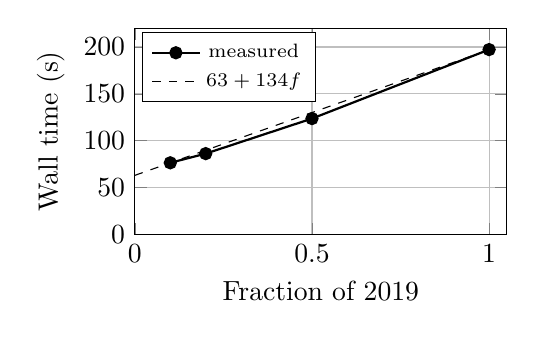
\begin{tikzpicture}
    \begin{axis}[width=0.52\columnwidth, height=4.2cm, xlabel={Fraction of 2019},
        ylabel={Wall time (s)}, xmin=0, xmax=1.05, ymin=0, ymax=220, grid=major,
        legend style={font=\scriptsize, at={(0.02,0.98)}, anchor=north west}]
      \addplot[mark=*, thick] coordinates {(0.1,76.4) (0.2,86.2) (0.5,123.6) (1.0,197.2)};
      \addlegendentry{measured}
      \addplot[dashed, domain=0:1] {63 + 134*x};
      \addlegendentry{$63+134f$}
    \end{axis}
  \end{tikzpicture}%
  \hfill
  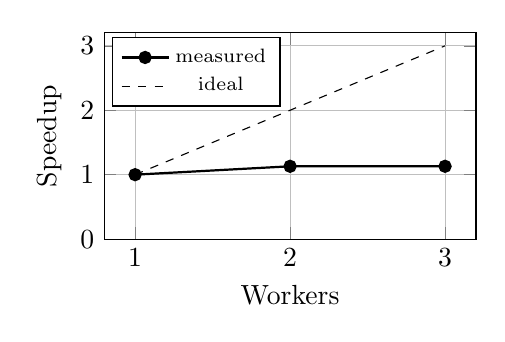
\begin{tikzpicture}
    \begin{axis}[width=0.52\columnwidth, height=4.2cm, xlabel={Workers},
        ylabel={Speedup}, xmin=0.8, xmax=3.2, ymin=0, ymax=3.2, xtick={1,2,3},
        grid=major, legend style={font=\scriptsize, at={(0.02,0.98)}, anchor=north west}]
      \addplot[mark=*, thick] coordinates {(1,1.00) (2,1.13) (3,1.13)};
      \addlegendentry{measured}
      \addplot[dashed, domain=1:3] {x};
      \addlegendentry{ideal}
    \end{axis}
  \end{tikzpicture}
  \caption{Left: wall time vs.\ input fraction (2 workers). Right: speedup vs.\ workers
  ($f=0.5$).}
  \label{fig:scaling}
\end{figure}

\paragraph{Why the speedup is far from ideal.}
\begin{itemize}
  \item \textbf{No extra hardware.} All workers are containers on the same 4-core laptop
    and the same SSD, so a new worker adds task slots but no cores. This shows in the scan
    stage: as the concurrent tasks go from 2 to 4 to 6, the median scan task goes from 7.0 to
    11.4 to 18.0\,s, so the stage only goes from 46.0 to 38.4 to 37.3\,s. With 6 slots the
    extra tasks run on hyperthreads of cores that are already busy.
  \item \textbf{Fixed partitioning.} The scan has 12 tasks (one per row group), i.e.\ 6, 3 and
    2 waves. Most of the other 40 stages have 1--12 small tasks and do not get faster with more
    slots.
  \item \textbf{Fixed overhead.} The driver plans and schedules 41 stages one operation after
    another; this part, like the fixed 63\,s above, does not shrink with more workers.
\end{itemize}
The run-to-run spread at $f=0.5$ is about $\pm$5\%, so 2 and 3 workers are equal. On a real
cluster, where each worker brings its own cores, disk and memory, we would expect the scan stage
to scale up to 12 slots; going further would need more input splits (files with several row
groups, or a \texttt{repartition} after the scan).


\section{Conclusion}
\label{sec:conclusion}

The pipeline produces all the required outputs over a year of data in 199\,s, against 342\,s for
the baseline, the largest gains did not come from configuration tuning, but from reading the
physical plans and applying the optimizations such as:
caching only the columns that are used, broadcasting the small side of a join
before the trip side is shuffled, and aggregating before joining, this should also be noted that
two of our assumptions were contradicted by the measurements, namely that a cache built from a
parquet scan would not need AQE to re-plan its partitioning, and that more workers would reduce
the execution time, both showed that in Spark, a change is only an optimisation once it is
measured. 
As future work, the same experiments should be repeated on a real cluster and over the
full dataset period, where the scan stage would be no longer be limited by the shared CPU cores.


\bibliographystyle{acm}
\bibliography{refs}

\end{document}
